\section{Experiments}
\label{sec:experi}

\subsection{Design}
\label{sec:experi:design}

Experiments to evaluate the performance of each file type and encoding were designed and executed. The dataset of FAST5 files used for these experiments was obtained by sequencing a genome sample from an adult male human on the ONT GridION. It's details are summarised in table \ref{tab:data}.

\begin{table}[h!]
    \caption{The dataset used for the experiments.\label{tab:data}}
    \begin{tabular}{|l|l|}
        \hline
        \textbf{Description} & Adult male human genome \\
        \hline
        \textbf{Sequencer} & ONT GridION \\
        \textbf{Sequencing time (days)} & 3 \\
        \hline
        \textbf{No.\nomenclature{No.}{Number} of base pairs (Gb\nomenclature{Gb}{Giga base pairs})} & 10.56 \\
        \textbf{No. of reads} & \num{496368} \\
        \textbf{Avg.\nomenclature{Avg.}{Average} read length (bp\nomenclature{bp}{Base pairs})} & \num{21278} \\
        \textbf{Max read length (bp)} & \num{1328419} \\
        \hline
    \end{tabular}
\end{table}

A list of read IDs representative of a typical analysis's order of read requests was generated by sorting the dataset's BAM file \cite{sam:file} by chromosome number and then by the base location on each chromosome. The result is a list of \num{534000} read IDs sorted by their genomic coordinates with \num{480004} being unique. This covers 96.7\% of the number of reads in the dataset, making it a robust list of read IDs for performance benchmarking.

The experiments were executed on a rack-mounted server capable of running up to 40 threads of execution in parallel. This amount is beneficial for observing the full relationship between performance and the number of threads used. It's specifications (table \ref{tab:server}) are typical for a small high performance computing (HPC\nomenclature{HPC}{High performance computing}) server which is usually available for genomics research scientists. The server's disk cache was also cleared before executing each experiment in order to prevent inaccurate I/O\nomenclature{I/O}{Input/output} results.

\begin{table}[h!]
    \caption{Specifications of the server used for the experiments.\label{tab:server}}
    \begin{tabular}{|l|l|}
        \hline
        \textbf{Description} & Dell PowerEdge C4140 Server Rack \\
        \hline
        \textbf{CPUs} & $2\, \times$ Intel Xeon Silver 4114 \\
        \textbf{CPU cores} & $2 \times 10$ \\
        \textbf{CPU threads} & $2 \times 20$ \\
        \hline
        \textbf{RAM\nomenclature{RAM}{Random-access memory}} & 376GB \\
        \textbf{Disk System} & 6.4TB NVMe drive \\
        \textbf{File System} & ext4 \\
        \textbf{OS\nomenclature{OS}{Operating system}} & Ubuntu 18.04.5 LTS\\
        \hline
    \end{tabular}
\end{table}

Two experiments were designed to evaluate performance. The first aimed to compare the size of each file type and encoding. Using the dataset's FAST5 files, equivalent SLOW5 files encoded in ASCII, binary and compressed binary were created. Each file's size was then measured in bytes using the Unix utility \textit{wc} \cite{wc}.

The second experiment aimed to compare the read access time of each file type and encoding using a varying number of threads. The motivation for varying the number of threads was to visualise the thread scalability issue from section \ref{sec:back} and how it was overcome in section \ref{sec:methods:multi}. For each file type and encoding, the total time taken to retrieve and store each read corresponding to the list of read IDs described in section \ref{sec:experi:design} was recorded. However, in order to reasonably compare the different encodings, each read was additionally transformed into the ASCII format which would be necessary in most user applications. This transformation time was also recorded, and was combined with the total read access time.

However, the file sizes and total read access times recorded by both experiments are specific for this dataset and list of read IDs. Hence, more normalised metrics were devised based on the number of base pairs in the dataset and corresponding reads of the list of read IDs. In particular, rather than comparing the raw file sizes, the average file size per base pair was used. And instead of comparing the total read access times, the average number of base pairs accessed per second was used.

\subsection{Results}
\label{sec:experi:results}

To benchmark the access time and file size of each format and encoding technique storing nanopore sequencing reads, experiments were performed on a sample of human DNA. A realistic list of read IDs was recorded from a sequencing pipeline and used to obtain the total access time for each format and encoding. Dividing the total number of reads by the total access time, we can obtain a normalised dataset-independent metric for comparing performance. Figure \ref{fig:time} plots this metric for each file type and encoding using the described dataset.

\begin{figure}[h]
    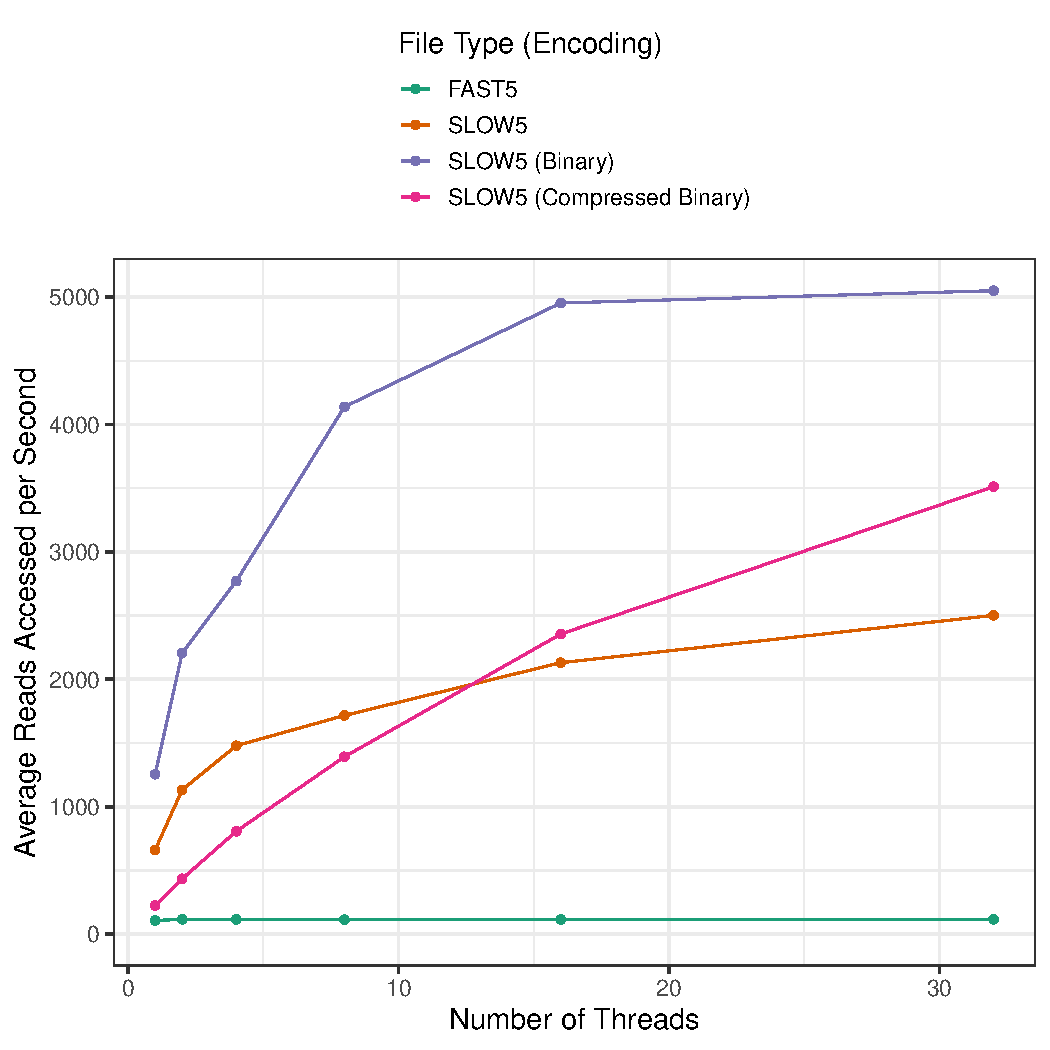
\includegraphics[width=\linewidth]{../../plots/gpgpu_read_time_thread.pdf}
    \caption{Number of reads accessed and transformed per second on average for each file format and encoding technique against the number of threads used.\label{fig:time}}
\end{figure}

A similar metric for comparing the space efficiency of each file type and encoding independent of datasets was devised by finding the size in bytes per read. Figure \ref{fig:size} was obtained on the aforementioned data and shows the size differences between each file type and encoding using this metric.

\begin{figure}[h]
    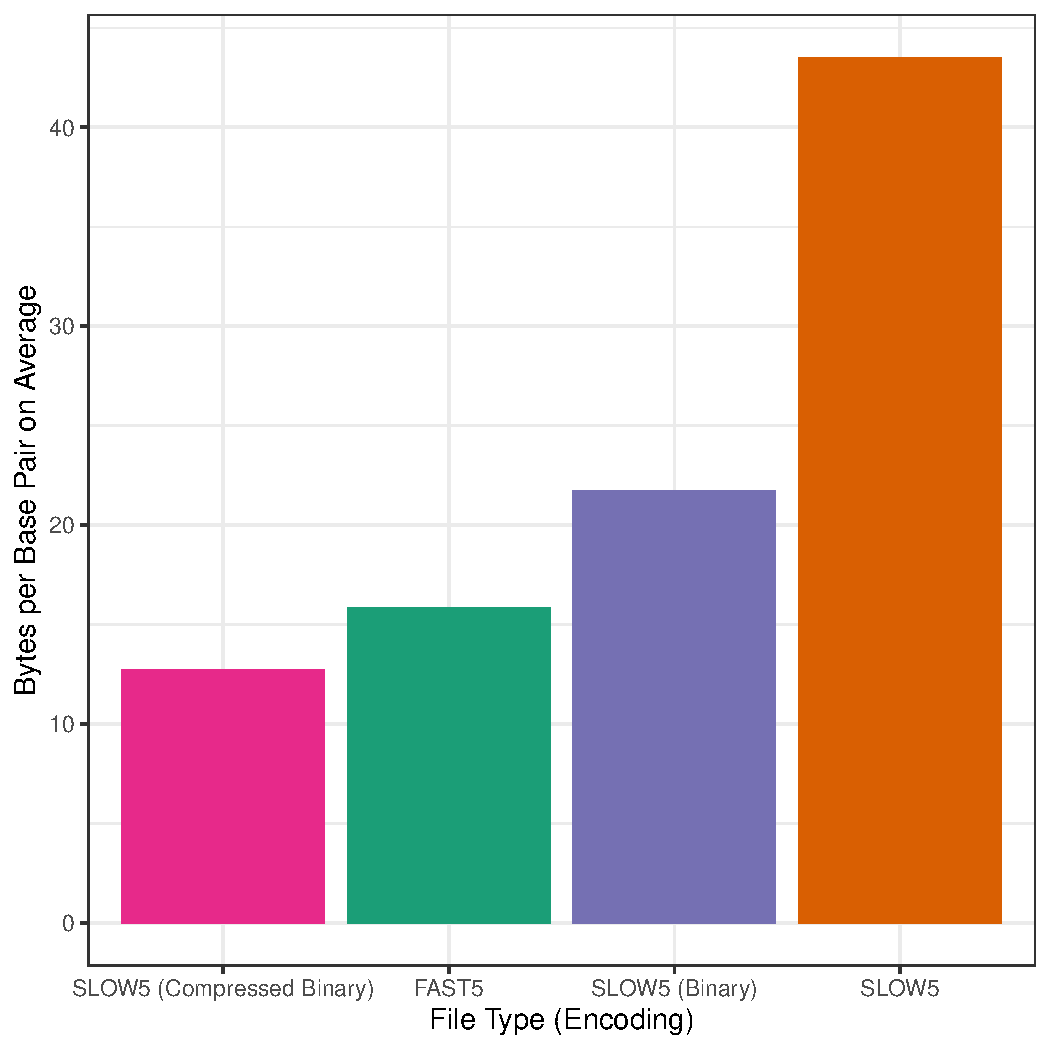
\includegraphics[width=\linewidth]{../../plots/gpgpu_size.pdf}
    \caption{Kilobytes stored per read on average for each file type and encoding technique.\label{fig:size}}
\end{figure}
